%% Copyright 2016 Nils Fleischhacker
%%
%% This work may be distributed and/or modified under the 
%% conditions of the LaTeX Project Public License, either 
%% version 1.3 of this license or (at your option) any later 
%% version. The latest version of this license is in
%%
%%   http://www.latex-project.org/lppl.txt
%%
%% and version 1.3 or later is part of all distributions of 
%% LaTeX version 2005/12/01 or later.
%%
%% This work has the LPPL maintenance status `maintained'.
%% 
%% The Current Maintainer of this work is Nils Fleischhacker.
%%
%% This work consists of the files tikzpeople.tex, tikzpeople.sty,
%% tikzpeople.shape.alice.sty, tikzpeople.shape.bob.sty, 
%% tikzpeople.shape.bride.sty, tikzpeople.shape.builder.sty,
%% tikzpeople.shape.businessman.sty, tikzpeople.shape.charlie.sty,
%% tikzpeople.shape.chef.sty, tikzpeople.shape.conductor.sty,
%% tikzpeople.shape.cowboy.sty, tikzpeople.shape.criminal.sty,
%% tikzpeople.shape.dave.sty, tikzpeople.shape.graduate.sty, 
%% tikzpeople.shape.groom.sty, tikzpeople.shape.guard.sty, 
%% tikzpeople.shape.jester.sty, tikzpeople.shape.judge.sty,
%% tikzpeople.shape.mexican.sty, tikzpeople.shape.nun.sty, 
%% tikzpeople.shape.nurse.sty, tikzpeople.shape.physician.sty,
%% tikzpeople.shape.pilot.sty, tikzpeople.shape.police.sty,
%% tikzpeople.shape.priest.sty, tikzpeople.shape.sailor.sty,
%% tikzpeople.shape.santa.sty and tikzpeople.shape.surgeon.sty
\documentclass{ltxdoc}
\usepackage[demo]{tikzpeople}
\usepackage[OT1]{fontenc}
\usepackage{hyperref}
\usepackage{microtype}
\usepackage{xspace}
\usepackage[most]{tcolorbox}
\usepackage[title]{appendix}
\usetikzlibrary{shapes.callouts}

\newcommand*{\Appendixautorefname}{Appendix}


\pgfdeclarelayer{background}
\pgfsetlayers{background,main}
\selectcolormodel{cmyk}

\newcommand{\tikzname}{Ti\emph{k}Z\xspace}

\newcommand{\varg}[1]{%
	{\ttfamily\char`\{}#1{\ttfamily\char`\}}}
\newcommand{\DescribeOption}[1]{\leavevmode
	\marginpar{\raggedleft\strut\MacroFont\string #1\ }}

\lstdefinestyle{example}{style=tcblatex,
  classoffset=0,
  texcsstyle=*\color{blue},%
  deletetexcs={begin,end},
  moretexcs={,%
    pgfdeclarehorizontalshading,pgfuseshading,node,
    useasboundingbox,draw}%
  classoffset=1,
  keywordstyle=\color{blue},%
  morekeywords={tikzpicture,shade,fill,draw,path,node,child,line,width,rectangle,minimum width,minimum size},
  classoffset=0}

\tcbset{%
  fillbackground/.style={before lower pre={%
  \tikzset{every picture/.style={execute at end picture={\begin{pgfonlayer}{background}
    \fill[yellow!15]
    ([xshift=-4mm,yshift=-4mm]current bounding box.south west) rectangle
    ([xshift=4mm,yshift=4mm]current bounding box.north east);
    \end{pgfonlayer}}}}}},
  explicitpicture/.style={before lower=\begin{center},after lower=\end{center},fillbackground}}

\newtcblisting{codeexample}[2][]{%
  enhanced,frame hidden,
  top=0pt,bottom=0pt,left=0pt,right=0pt,arc=0pt,boxrule=0pt,
  colback=blue!15,
  listing style=example,
  sidebyside,text and listing,text outside listing,sidebyside gap=2mm,
  lefthand width=#2,tikz lower,fillbackground,
  #1}

\title{\tikz{\node[graduate,shield,sword,minimum height=2cm]{}}\\The \textsf{tikzpeople} package}
\author{Nils Fleischhacker}
\date{}

\begin{document}
\maketitle

\begin{abstract}
  This package provides people shaped pgf-shapes to be used in \tikzname pictures.
  Given that the the only thing this package does is providing new node shapes for \tikzname, it should probably be a \tikzname library.
  It isn't, it's a package instead, so deal with it.
  
  The package probably has many problems and is nowhere near optimal, but if you find it useful, feel free to use it anyway.
\end{abstract}

\section{Introduction}
	Let me start with a word of warning: 
	The node-shapes defined by this package are heavily influenced by a type of clip art included in the \textsf{Microsoft Visio} software.
	I am by no means an expert on copyright law and as such can make no claim under which circumstances using these shapes might infringe on Microsoft's copyright.
	I do not expect that there are any problems, but be aware of this.
	Let's consider this package an homage to the great design of those \textsf{Visio} clip arts and get on with our lives.
	\subsection{Intended Usecase}
		If you are confused about any of the packages design choices, the original use-case the package was written for might serve as an explanation.
		The package was originally written to provide me with shapes of people to depict parties in cryptographic protocols and security definitions on beamer slides.
		An example of this can be seen in \autoref{fig:protocolexample}.
		\begin{figure}
			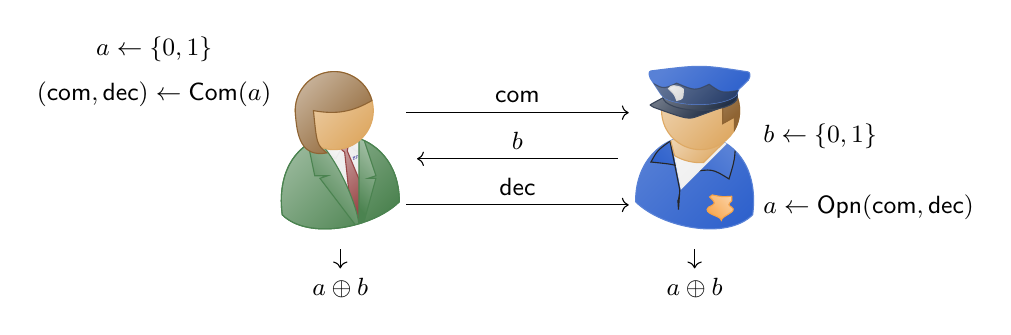
\begin{tikzpicture}[font=\small]
				\node[businessman,female,minimum size=1.5cm] (A) {};
				\node[police,right=3cm of A,minimum size=1.5cm,mirrored] (B) {};
				\node[anchor=north east] at (A.north west) (a2) {$(\mathsf{com},\mathsf{dec}) \gets \mathsf{Com}(a)$};
				\node[anchor=south] at (a2.north) (a1) {$a\gets\{0,1\}$};
				\node[anchor=south west] at (B.south east){$a \gets \mathsf{Opn}(\mathsf{com},\mathsf{dec})$};
				\draw (A.35) edge[->] node[above] {$\mathsf{com}$} (B.145);
				\node[anchor=south west] at (B.east |- B.180) {$b\gets\{0,1\}$};
				\draw (A.0) edge[<-] node[above] {$b$} (B.180);
				\draw (A.325) edge[->] node[above] {$\mathsf{dec}$} (B.215);
				\draw (A.270) ++(0,-.5) node {$a\oplus b$} edge[<-] (A.270);
				\draw (B.270) ++(0,-.5) node {$a\oplus b$} edge[<-] (B.270);
			\end{tikzpicture}
			\caption{A secure coin flipping protocol constructed from bit commitment.}
			\label{fig:protocolexample}
		\end{figure}
		If this intended use-case does not resolve your confusion with any weird behavior or design choice, then chances are good that I made a mistake or just did not know any better.
		If you spot a mistake or know how to do something in a saner way, shoot me a message to let me know.

\subsection{Installation}
	To install the package just drop the \textsf{tikzpeople.sty} file and all the shape files, i.e. \textsf{tikzpeople.shape.\meta{shapename}.sty}, somewhere \LaTeX can find them.
	You might for example put them in your local \textsf{texmf} tree at \url{\textasciitilde/texmf/tex/latex/tikzpeople/}.
	Alternatively simply drop all the files into the folder where your main \textsf{.tex} file resides.\footnote{Do not use a subfolder. While you can refer to the package itself in a hackish way using a relative path, \LaTeX wont be able to find the shape files.}

\section{Usage}
	To use the \textsf{tikzpeople} shapes, just write |\usepackage|\oarg{options}\varg{tikzpeople} somewhere in the preamble of your document.
\subsection{Package Options}
	The package has three global options.
	\DescribeOption{draft}
	Compiling a document with many \textsf{tikzpeople} nodes can be very slow.
	This is especially true for some of the node shapes that make heavy use of \tikzname decorations.
	To make documents compile faster during the drafting stage, the |draft| option is available.
	In draft mode all \textsf{tikzpeople} nodes are only drawn as simple outlines. 
	\makeatletter
	\let\listbackup\tikzpeople@shapelist
	\@tikzpeople@drafttrue
	\let\tikzpeople@alice@paint\relax
	\let\tikzpeople@alice@painthair\relax
	\let\tikzpeople@alice@paintshirtdetails\relax
	\let\tikzpeople@alice@definecolors\relax
	\let\tikzpeople@alice@definestyles\relax
	\let\tikzpeople@alice@colors\relax
	\tikzpeople@declareshape{alice}
	\begin{codeexample}{3cm}
\node[alice,minimum size=1.5cm] {Alice};
	\end{codeexample}
	\@tikzpeople@draftfalse
	\let\tikzpeople@alice@paint\relax
	\let\tikzpeople@alice@painthair\relax
	\let\tikzpeople@alice@paintshirtdetails\relax
	\let\tikzpeople@alice@definecolors\relax
	\let\tikzpeople@alice@definestyles\relax
	\let\tikzpeople@alice@colors\relax
	\tikzpeople@declareshape{alice}
	\let\tikzpeople@shapelist\listbackup
	\makeatother
	
	\DescribeOption{demo}
	The |demo| option loads the package in demo mode, introducing additional commands.
	These commands |\alltikzpeople| and |\tikzpeoplecolors| explained below are not meant for productive use.
	They are useful for showcasing the available shapes with different node options and getting information for customizing colors.
	
	\DescribeOption{nobeards}
	The |nobeards| option removes all beards from \textsf{tikzpeople} nodes.
	In particular, \textsf{tikzpeople} marked as evil no longer have goatees.
	This option exists because I have been informed that having evil \textsf{tikzpeople} with goatees is very insensitive and discriminatory against people with goatees.
	For a little bit of petty defiance, this option also removes Santa's beard.

	\DescribeOption{saturated}
	The \textsf{saturated} option causes all nodes to be rendered with saturated colors.
	Standard nodes are rendered with somewhat washed out colors.
	This works well on light backgrounds but can look weird on dark background.
	The |saturated| option can also be used on individual nodes.
	
\subsection{Available Shapes}
	Once the package is loaded, any of the defined shapes can be used as the shape of any \tikzname node just like any other predefined shape.
	\begin{codeexample}{3cm}
\node[draw,rectangle,minimum size=1.5cm] at (0,2) {};
\node[businessman,minimum size=1.5cm] at (0,0) {};
	\end{codeexample}
	However, it should be noted that in many respects the nodes behave quite differently from standard node shapes.
	First, the nodes are drawn and filled, whether |draw| and |fill| are specified or not, because -- quite frankly -- if you do not want to draw the node, then the \textsf{tikzpeople} are quite useless to you.
	Another area where the behavior might be unexpected to the experienced \tikzname user is concerning the node text.
	\begin{codeexample}{3cm}
\node[draw,rectangle,minimum size=1.5cm] at (0,2) {A Rectangle};
\node[businessman,minimum size=1.5cm] (B) at (0,0) {A Businessman};
\draw[gray,dotted] (B.north west) rectangle (B.south east);
	\end{codeexample}
	The text appears below the actual node, not within and the width of the text influence neither the drawn shape nor any of the border anchors.
	The reason for this is that in the intended usecase, the node text -- if present at all -- is simply a label and is not supposed to influence the size or behavior of the node.
	
	Another oddity of the tikzpeople shapes is that the border anchors and size of the node only takes into consideration the underlying shape of a person, and nothing of the -- sometimes much larger -- stuff such as hats added by some of the shapes.
	\begin{codeexample}{3cm}
\node[person,minimum size=1.5cm] (B) at (0,4) {A Person};
\draw[gray,dotted] (B.north west) rectangle (B.south east);
\node[mexican,minimum size=1.5cm]     (M) at (0,0) {A Mexican};
\draw[gray,dotted] (M.north west) rectangle (M.south east);
	\end{codeexample}
	Again, the reason for this is that two shapes specified to have the same size, should behave like two people of same size.
	If for example \texttt{minimum width} would take the actual width into consideration, then the Mexican would be much smaller than the person.
	
	While all of these oddities are useful to me and in my specific usecase, they may cause problem for you in any number of ways.
	So if you don't think you will be able to cope with them, I suggest you stop reading and look elsewhere for people-shaped \tikzname nodes.

\subsection{The Available Shapes}
	\DescribeMacro{\alltikzpeople} If the package is loaded with the |demo| option, all provided shapes can easily be viewed using the |\alltikzpeople|\allowbreak\marg{width}\allowbreak\marg{options} command.
	The command takes two arguments. 
	The first argument specifies the |minimum size| of the drawn nodes in centimeters, the second argument is a comma separated list of options passed to each node.
	The command then produces figures such as \autoref{fig:tikzpeoplefigure1} and \autoref{fig:tikzpeoplefigure2}, which were produces using the command |\alltikzpeople|\varg{1.5}\varg{}
	\DescribeMacro{\alltikzpeople*} The starred version of the command does exactly the same but omits the name of the shapes.
	\alltikzpeople{1.5}{}
\subsection{General Node Options}
	A number of options can be used to influence the appearance of \textsf{tikzpeople}.
	These options are explained here in alphabetical order.
	Not all nodes are affected by all options.
	This is the case if the option is either simply not applicable or if I have not found a way to make is look not weird.
	
	\DescribeOption{evil}	The |evil| option is supposed to make nodes look more evil than usual.
	For most tikzpeople this is accomplished by adding horns and a goatee.
	\begin{codeexample}{3.2cm}
\node[priest,minimum size=1cm,xshift=-1.2cm]{};
\node[priest,evil,minimum size=1cm] {};
	\end{codeexample}
	This is especially useful to depict attackers in a cryptographic or security setting.
	Unaffected by this option are: \texttt{guard,santa,devil}.
	The color of the horns is controlled with the |horns| key.

	\DescribeOption{female}	The |female| option is supposed to make stereotypically male nodes look just a tad more feminine.
		For most tikzpeople this is accomplished by adding longer hair and losing the beard -- though surprisingly, evil women still tend to have a goatee.
		\begin{codeexample}{3.2cm}
\node[conductor,minimum size=1cm,xshift=-1.2cm]{};
\node[conductor,female,minimum size=1cm]{};
		\end{codeexample}
		This is useful to avoid being called sexist for not having women in you figures.
		On the other hand people can now accuse you of enforcing gender stereotypes. So have fun.
		Unaffected by this option are: \texttt{alice, bride, guard, judge, nun, pilot}.

	\DescribeOption{good}	The |good| option is supposed to make nodes look extraordinarily good.
		For most tikzpeople this is accomplished by adding a halo.
		\begin{codeexample}{3.2cm}
\node[sailor,minimum size=1cm,xshift=-1.2cm]{};
\node[sailor,good,minimum size=1cm]{};
		\end{codeexample}
		This could be useful to, e.g., depict a trusted party in a security context.
		Unaffected by this option are: \texttt{guard, mexican, santa}.
		The color of the halo is controlled with the |halo| key.
		
	\DescribeOption{mirrored}	The \textsf{mirrored} option makes nodes face to the left instead of the right.
		\begin{codeexample}{3.2cm}
\node[graduate,minimum size=1cm,xshift=-1.2cm]{};
\node[graduate,mirrored,minimum size=1cm]{};
		\end{codeexample}
		I'm sure you will figure out the usefulness of this option on you own.

	\DescribeOption{monitor} The \textsf{monitor} option draws a monitor in front of the node.
		\begin{codeexample}{4cm}
\node[judge,minimum size=1cm,xshift=-1.2cm]{};
\node[judge,monitor,minimum size=1cm]{};
		\end{codeexample}
		This could be useful to emphasize that parties are actually using a computer and not doing complex computations in their head.
	
	\DescribeOption{saturated} The \textsf{saturated} option causes the node to be rendered with saturated colors.
		\begin{codeexample}{3.2cm}
\node[pilot,minimum size=1cm,xshift=-1.2cm]{};
\node[pilot,saturated,minimum size=1cm]{};
		\end{codeexample}
		Standard nodes are rendered with somewhat washed out colors.
		This works well on light backgrounds but can look weird on dark background.
		The |saturated| option can also be used as a global package option.

	\DescribeOption{shield} The \textsf{shield} option gives the node a shield.
		\begin{codeexample}{4cm}
\node[alice,minimum size=1cm,xshift=-1.2cm]{};
\node[alice,shield,minimum size=1cm]{};
		\end{codeexample}
		This could be useful to symbolize that a party is defending something and combines well with the |sword| option.
		The colors of the shield are controlled using the keys |shieldmid|, |shieldedge|, and |shieldrivets|.
	
	\DescribeOption{sword} The \textsf{sword} option gives the node a sword.
		\begin{codeexample}{4cm}
\node[dave,minimum size=1cm,xshift=-1.2cm]{};
\node[dave,sword,minimum size=1cm]{};
		\end{codeexample}
		This could be useful to symbolize that a party is attacking or defending something and combines well with the |shield| option.
		The colors of the sword are controlled using the keys |swordblade|, |swordguard|, |swordpommel|, and |swordgrip|.

	All of these options can be arbitrarily combined. So, e.g., |good| \textsf{tikzpeople} can very well be |evil| at the same time.
	\begin{codeexample}{4cm}
\node[chef,evil,female,good,mirrored,monitor,
  saturated,shield,sword,minimum size=1.5cm]{};
	\end{codeexample}
\subsection{Color Options}
	Almost all the colors used in the \textsf{tikzpeople} shapes can be specified separately.
	So if you feel, that you do not need a simple priest, but a cardinal instead, just take the priest, make the shirt and hat red and give him gray hair and we have a decent approximation of a cardinal.\footnote{In my defense, I'm not catholic, so I might be missing something crucial about cardinals. Rest assured that I meant no disrespect.}
	\begin{codeexample}{3cm}
\node[priest, shirt=red, hat=red, hair=gray, minimum size=1.5cm]{};
	\end{codeexample}
	Similarly, maybe what we actually need is a monk.\footnote{Again, I do not know much about monks...}
	\begin{codeexample}{3cm}
\node[priest,shirt=brown, hat=skin, cross=gray, collar=brown, minimum size=1.5cm]{};
	\end{codeexample}
	What I'm trying to get across is, using changes in coloring, we get tons of additional options for different kinds of \textsf{tikzpeople} we can draw.
	
	\DescribeMacro{\tikzpeoplecolors} If the package is loaded with the |demo| option, you can use the command |\tikzpeoplecolors|\marg{shapename} to produce a figure giving you an idea, which color keys can be used for which shape.
	For your convenience, all of those figures are included in \autoref{app:colors}.
	
	\subsection{Text Options}
	Some \textsf{tikzpeople} have include customizable text, such as the |businessman|'s monogram.
	These texts can be specified with pgfkeys just as with the color options.
	\vspace{.75em}
	\begin{codeexample}{3cm}
\path [clip] (0cm,1cm) rectangle (1.5cm,-1cm);
\node[businessman, monogramtext=ER ,minimum size=5cm]{};
	\end{codeexample}
	
	\vspace{1em}
	
	All texts are scaled to fit the available space. Specifying significantly longer text will therefore cause it to be unreadable.
	
	\DescribeOption{monogramtext} The |monogramtext| option is available for |businessman| shapes and changes the text of the monogram.
	While you can change the monogram to any arbitrary text, you should be aware that the monogram is rendered as |\mathcal| and anything except for uppercase letters will probably lead to unexpected results.
	
	\DescribeOption{badgetext} The |badgetext| option is available for |nurse| shapes and changes the text printed on the badge.
	
\subsection{Anchors}
		\tikzset{shape example/.style={color=black!30, draw, fill=yellow!30, minimum size=3cm}}
		\begin{figure}[htp]
		\centering
		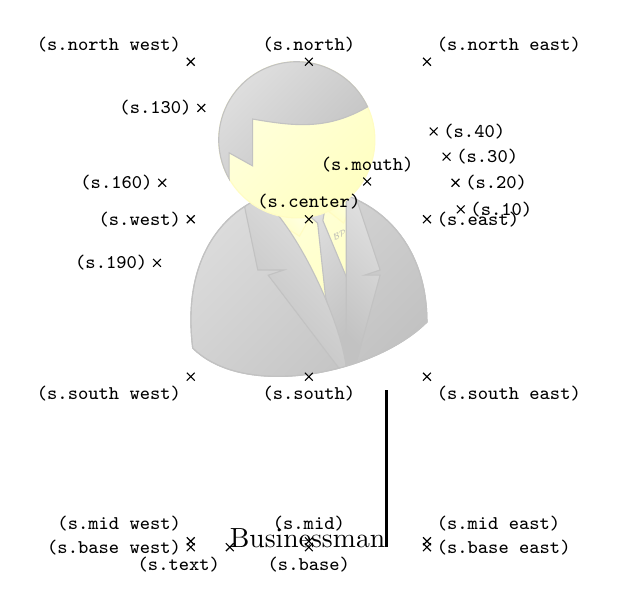
\begin{tikzpicture}
			\node[name=s,shape=businessman,minimum width=3cm,skin=yellow!30!,hair=black!30!,tie=black!30!,undershirt=yellow!30!,shirt=black!30!,monogram=black!30!] {Businessman\vrule width 1pt height 2cm};
			\foreach \anchor/\placement in
				{north west/above left, north/above, north east/above right,
				west/left, center/above, east/right,				
			mid west/above left, mid/above, mid east/above right,
			base west/left, base/below, base east/right,
				south west/below left, south/below, south east/below right,
				text/below left, 10/right, 20/right, 30/right, 40/right, 130/left, 
				160/left, 190/left, mouth/above}
				\draw[shift=(s.\anchor)] plot[mark=x] coordinates{(0,0)}
					node[\placement] {\scriptsize\texttt{(s.\anchor)}};
		\end{tikzpicture}
		\caption{Anchors of a \texttt{businessman} tikzpeople shape.}
		\label{fig:anchors1}
	\end{figure}
	\begin{figure}[htp]
		\centering
		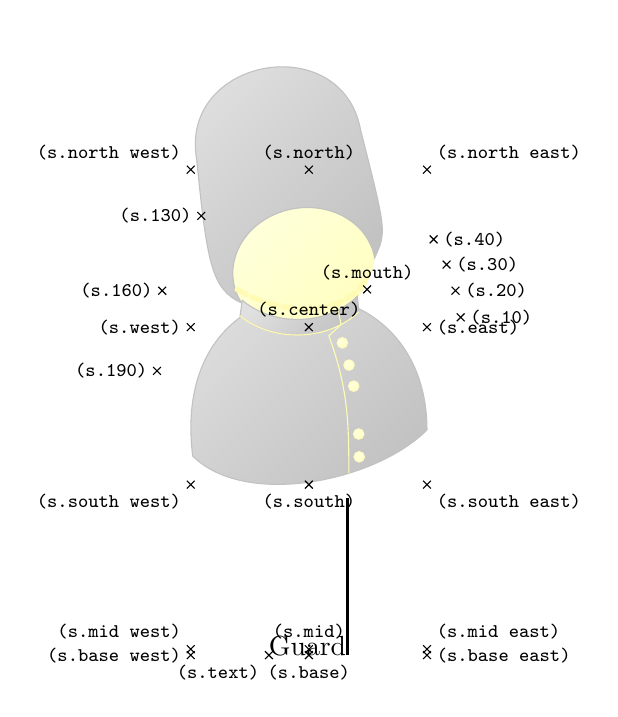
\begin{tikzpicture}
			\node[name=s,shape=guard,minimum width=3cm,skin=yellow!30!,hat=black!30!,lining=yellow!30!,details=yellow!30!,shirt=black!30!,collar=black!30!] {Guard\vrule width 1pt height 2cm};
			\foreach \anchor/\placement in
				{north west/above left, north/above, north east/above right,
				west/left, center/above, east/right,				
			mid west/above left, mid/above, mid east/above right,
			base west/left, base/below, base east/right,
				south west/below left, south/below, south east/below right,
				text/below left, 10/right, 20/right, 30/right, 40/right, 130/left, 
				160/left, 190/left, mouth/above}
				\draw[shift=(s.\anchor)] plot[mark=x] coordinates{(0,0)}
					node[\placement] {\scriptsize\texttt{(s.\anchor)}};
		\end{tikzpicture}
		\caption{Anchors of a \texttt{guard} tikzpeople shape.}
		\label{fig:anchors2}
	\end{figure}
	Basically all standard anchors for nodes exist also for tikzpeople nodes.
	However, as mentioned before, most of them are not influenced by the node text.
	Basically the only anchors that depend on the node text are the |text|, |base|, and |mid| anchors.
	Furthermore, the anchors only take into account the basic shape of the person, not any of the -- possibly much larger -- additions such as hats.
	As a reference, \autoref{fig:anchors1} and \autoref{fig:anchors2} show all the anchors of |businessman| and |guard| nodes.
	
	A special anchor is the |mouth| anchor. In conjunction with \tikzname's |callout| shapes this anchor allows to easily depict talking \textsf{tikzpeople}..
	\begin{codeexample}{4.6cm}
\node[name=a,shape=police,minimum size=1cm,xshift=-1.25cm] {};
\node[name=b,shape=criminal,minimum size=1cm,mirrored,xshift=1.25cm] {};
\node[ellipse callout, draw,yshift= .3cm, callout absolute pointer={(a.mouth)}, font=\tiny] {Hey!};
\node[ellipse callout, draw, yshift=-.3cm, callout absolute pointer={(b.mouth)}, font=\tiny] {What?};
	\end{codeexample}

\subsection{Messing with PGF Internals}
When using several of the |decoration| heavy \textsf{tikzpeople}, the package runs into errors in the internals of |pgf|.
Namely into ``Dimension to large'' errors in the |\pgfmath@function@veclen| command.
Apparently this happens because we are working with numbers that are too small.
As per this \TeX-stackexchange answer \url{http://tex.stackexchange.com/a/20888/15636}, \textsf{tikzpeople} redeclares |\pgfmath@function@veclen| with a fixed version.


\clearpage
\begin{appendices}
	\section{Color Options}
		\label{app:colors}
		\tikzpeoplecolors{alice}
		\vfill\tikzpeoplecolors{bob}
		\vfill\tikzpeoplecolors{bride}
		\vfill\tikzpeoplecolors{builder}
		\vfill\tikzpeoplecolors{businessman}
		\vfill\tikzpeoplecolors{charlie}
		\vfill\tikzpeoplecolors{chef}
		\vfill\tikzpeoplecolors{conductor}
		\vfill\tikzpeoplecolors{cowboy}
		\vfill\tikzpeoplecolors{criminal}
		\vfill\tikzpeoplecolors{dave}
		\vfill\tikzpeoplecolors{devil}
		\vfill\tikzpeoplecolors{duck}
		\vfill\tikzpeoplecolors{graduate}
		\vfill\tikzpeoplecolors{groom}
		\vfill\tikzpeoplecolors{guard}
		\vfill\tikzpeoplecolors{jester}
		\vfill\tikzpeoplecolors{judge}
		\vfill\tikzpeoplecolors{maninblack}
		\vfill\tikzpeoplecolors{mexican}
		\vfill\tikzpeoplecolors{nun}
		\vfill\tikzpeoplecolors{nurse}
		\vfill\tikzpeoplecolors{physician}
		\vfill\tikzpeoplecolors{pilot}
		\vfill\tikzpeoplecolors{police}
		\vfill\tikzpeoplecolors{priest}
		\vfill\tikzpeoplecolors{sailor}
		\vfill\tikzpeoplecolors{santa}
		\vfill\tikzpeoplecolors{surgeon}
	\end{appendices}
\end{document}

